The TUE \acrfull{ed} is a \acrfull{ros} based 3D geometric, object-based world representation system for robots. In itself \acrshort{ed} is database system that structures multi-modal sensor information and represents this in an object-based world representation that can be utilized for robot localization, navigation, manipulation and interaction functions. See Figure \ref{fig:ed} for a schematic overview of \acrshort{ed}. \footnote{\acrshort{ed} is an evolution of \acrfull{wire} that was created in the FP7 RoboEarth Project. Secondly, the Environment Descriptor is utilized within the RoboCup @home competition (also read the TU/e 2015 technical description paper for RoboCup). More information,  software, installation manual and tutorial can be found on \url{https://github.com/tue-robotics/ed}}
Moreover, ED is used as extension of the ROS middle ware and is necessary to execute efficient collaboration between multiple robots.  ED allows multiple robots to use and update the same world model. Static and dynamic objects in the environment space are shared which allows ‘easy’ cooperation when if for example comes to picking up objects. Robot-Robot task distribution can easily be distributed without the need of additional communication protocol that translates the perception of on robot to the other.
\begin{figure}[ht]
	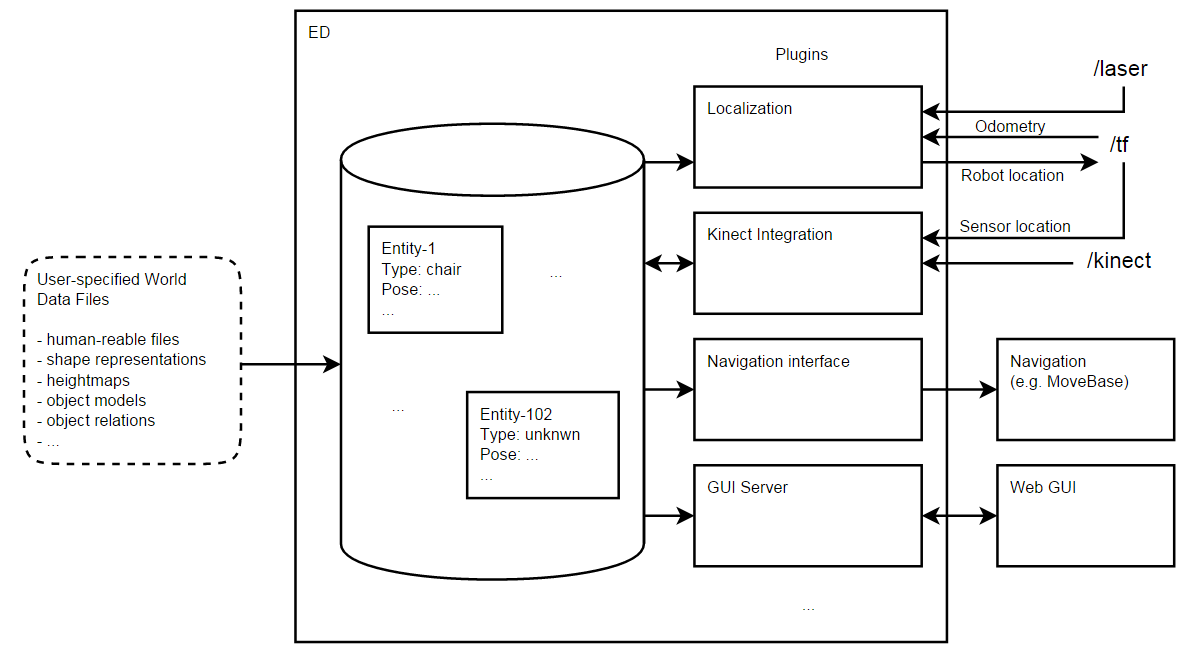
\includegraphics[width = \linewidth]{Figures/ed_overview}
	\caption{schematic overview of TUE Environment Descriptor.}
	\label{fig:ed}
\end{figure}
\acrshort{ed} is one re-usable environment description that can be used for a multitude of needed functionalities. Instead of having different environment representations for localization \acrfull{amcl}, navigation (MoveBase \footnote{\url{http://wiki.ros.org/move_base}}), manipulation (MoveIt!\footnote{\url{http://moveit.ros.org/}}), interaction, etc. An improvement in this single, central world model will reflect in the performances of the separate robot capabilities. It omits updating and synchronization of multiple world models. At the moment different \acrshort{ed} modules exist which enable robots to localize themselves, update positions of known objects based on recent sensor data, segment and store newly encountered objects and visualize all this through a web-based \acrshort{gui}.
\begin{figure}[ht]
	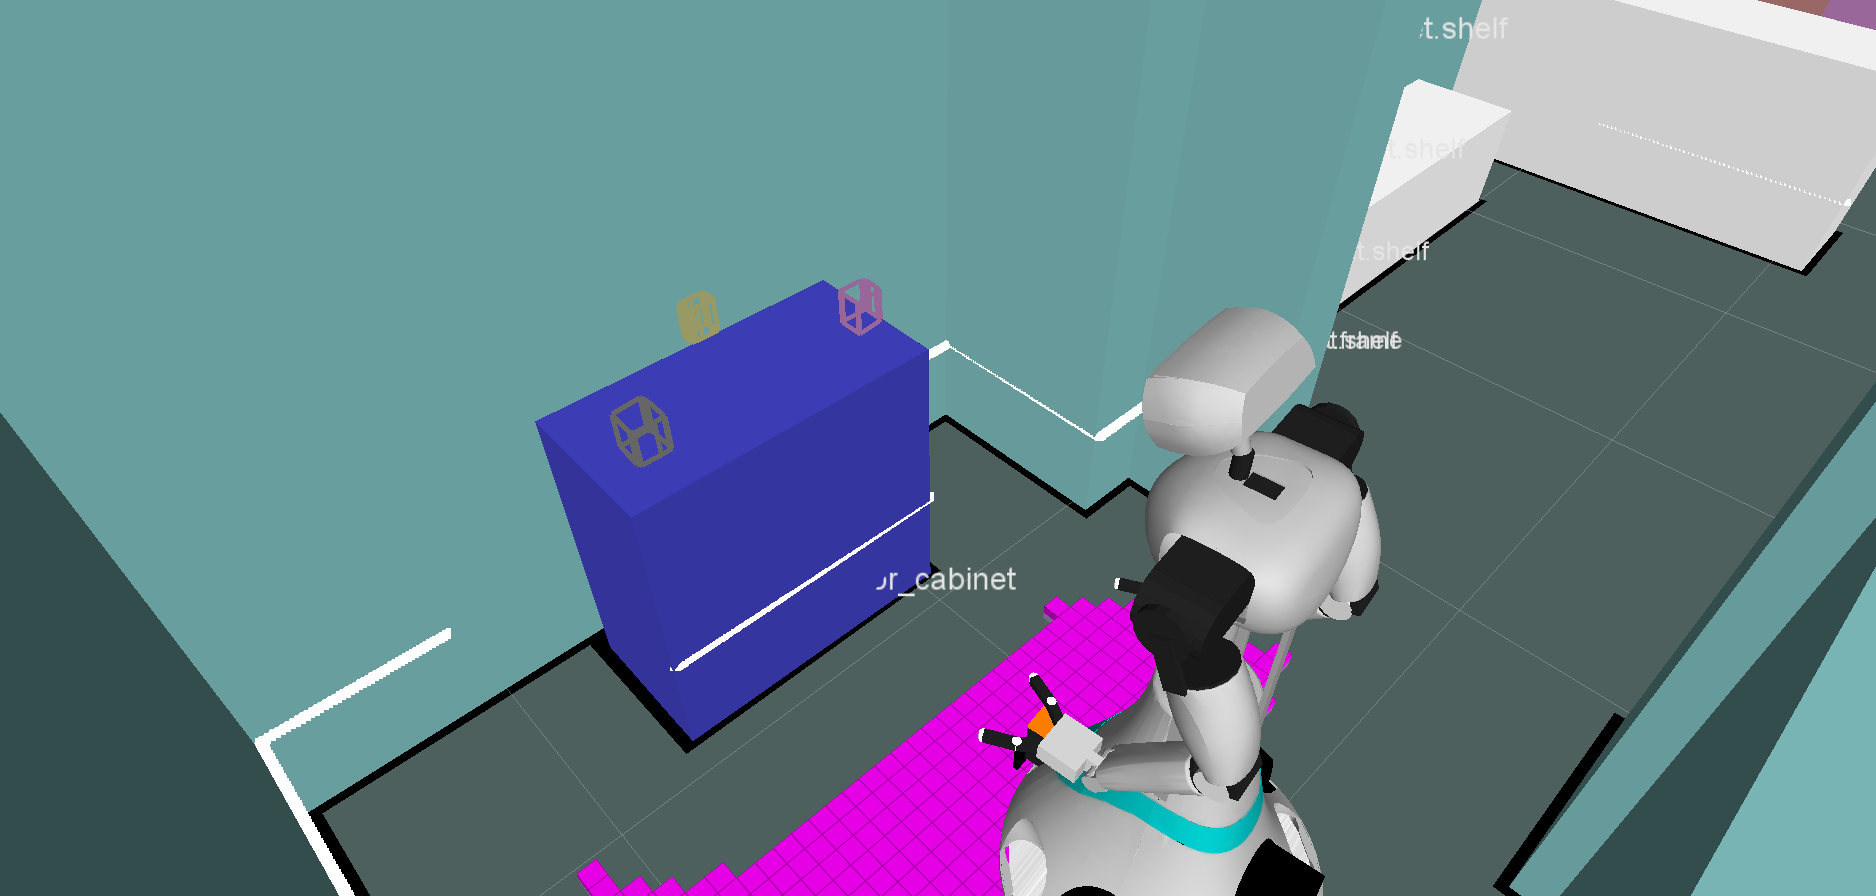
\includegraphics[width = \linewidth]{Figures/ed_segmentation}
	\caption{A view of the world model created with ED. The figure, show the occupation grid as well as (unknown) objects recognized on top of the cabinet.}
	\label{fig:ed_segmentation}
\end{figure}
